\chapter{Linked Data}
\label{ch5}

\section{Weaving a Web of Data}



The architects  of the World Wide Web made some very specific choices in its design 
to allow it to grow to global scale.   The  Web relies on open standards to specify the components of its
architecture, allowing them to span different software and hardware, making it both implementation-independent and domain-independent. To
support a Web of data, we want to take advantage of this infrastructure as much as possible. 
By
reusing  the World Wide Web architecture, the Web of data
becomes a backward-compatible extension and evolution of the hypertext
Web and remains compatible and combinable with all the other facets of
it. The Web of data applies the Web architecture to structured data
sharing on a World Wide scale. Meanwhile, it retains its architectural
support for decentralization, extensibility and openness.


What changes do we have to make to the hypertext Web to allow the Web of data
to be able to describe  resources and publish data? As
shown in Figure~\ref{fig:ch5.1}, this requires two steps:  expanding the set of exchange formats from     HTML (and other document formats) to include  RDF and its serializations (Section~\ref{serialization}) for exchanging data, and generalizing 
URLs (Uniform Resource Locators) to URIs (Uniform Resource Identifiers) 
or IRIs (Internationalized resource identifiers), to identify and then describe virtually anything. ,

\begin{figure}
    \centering
    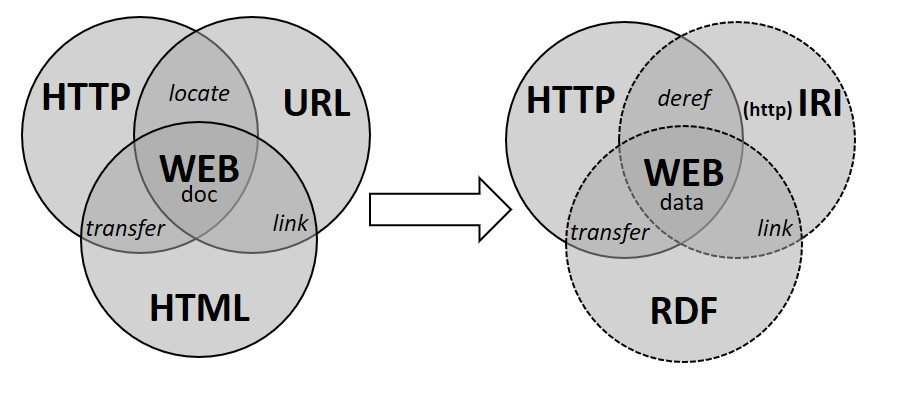
\includegraphics[width=5.0in]{media/ch5/figure-05-01.jpg}
    \caption{Relying on the Web architecture to publish linked data}
    \label{fig:ch5.1}
\end{figure}


\subsection{A Web of Data vs Data on the Web}

We can put data on the web simply by making a spreadsheet or even a PDF available on
a web page somewhere.    A Web of data, in contrast, consists of data from around the world that is linked together so that it can be found, browsed,
crawled, integrated, etc. In a Web of data, the core idea is \emph{linked data}, i.e. data sets (and data elements in them)  linked across the
World Wide Web in the same way Web pages, Web sites and anchored texts
are linked across the World on the Web. Instead of just
using HTML to write Web pages that include links to other pages, the Web of
data uses RDF to write data descriptions that include links to other data
descriptions.

Tim Berners-Lee introduced best practices for linked data in his
personal notes on Linked Data Design Issues \cite{linkeddatadesign}, stating the
architectural principles and explaining the thinking behind the linked data
specifications.  These ideas were extended and documented in \cite{heath2011linked}.  In this chapter, we will explain in detail his three rules 
for data publication that will allow us to weave a web of data:



\begin{enumerate}
\def\labelenumi{\arabic{enumi}.}
\item
\label{ruleURI}
  Use HTTP URIs to name everything: Just as URLs were introduced to
  address and locate resources on the Web, the Web of data uses URIs to
  name the things it describes. But by using HTTP URIs we can also
  provide a default mechanism to obtain descriptions: HTTP URIs are
  names (URIs) supporting lookup (HTTP access). This allow us to
  look up the name of the things they identify.\footnote{For added security,
  most web sites today use a more secure version of the HTTP protocol, called HTTPS. 
  For the purposes of this book, when we refer to a "HTTP URI", we include URIS
  that use the HTTP protocol.}
\item
\label{ruleFYN}
  When an agent accesses an HTTP URI, the server must provide descriptive
  information about the resource identified by that URI using the Web
  standard languages, in particular RDF and its syntaxes.
\item
\label{ruleLink}
  In the descriptive data it provides, a server must include links to
  HTTP URIs of other things so that Web clients can discover more things
  by looking up these new HTTP URIs recursively at will.
\end{enumerate}

These simple rules are a natural extension of how thy hypertext Web works. When we put a hypertext page 
on the web, use an HTTP URI (URL) to reference it.  When an agent accesses that HTTP URI, the server provides 
the page itself.  A hypertext page refers to other pages by including links to their HTTP URIs. 
For the hypertext web, this makes the pages interconnected; from any page an 
information consumer can access others.

By applying these  rules to the Web of data, we make it interconnected in the same way.  
when we use an HTTP URI   for our data elements (rule \ref{ruleURI}), 
we make it possible for anyone on the web to reference them. Once someone
(re-)uses one of our HTTP URIs , their data set and ours
are interconnected.  When we include links in our data to 
other data sets (rule \ref{ruleLink}) and  describe our own 
data sets (rule \ref{ruleFYN}), we make 
the interconnected data \emph{discoverable}, that is, 
someone coming to one data set can discover another
without having to search for it. 


\hypertarget{calling-a-cat-an-httpcat}{%
\subsection{Calling a cat an
http://cat}\label{calling-a-cat-an-httpcat}}

When we expand the hypertext web into a full Web of data, instead of just using URLs to 
identify what exists on the web (\url{http://my-site.fr}), we also start using
URIs to identify, on the web, what exists in general
(e.g., \url{http://animals.org/cat\#mytsie}, for Fabien's cat, Mytsie).  As we include IRIs in the Web of data, we identify,
on the web, what exists, in any language
\setcode{utf8}
(e.g., http://\<الحيوانات.tn/ >.tn/\begin{CJK*}{UTF8}{gbsn}猫
\end{CJK*}\#mytsie).



The distinction between identifying what is on the Web vs. identifying
on the Web anything that exists, is much more than a play on words.
Instead of just using the Web to exchange data about its own content, we
can use it to exchange data about anything around us: a page, a person,
a car, a cat, an idea, a country, a product, a service, a policy, a
relation, etc.

In the acronyms URL, URI and IRI the `R' stands for ``Resource''. In the
Web architecture a resource is anything that can be identified. And in
practice, URIs are now used to name a lot of very different things. Here
are some examples:

\begin{itemize}
\item
  URI for Paris in DBpedia: \url{http://dbpedia.org/resource/Paris}
\item
  URI for the protein MUC18 in UniProt:
  \url{http://www.uniprot.org/uniprot/P43121}
\item
  URI for the name of Victor Hugo in the Library of Congress:
  \url{http://id.loc.gov/authorities/names/n79091479}
\item
  URI for Xavier Dolan in Wikidata:
  \url{http://www.wikidata.org/entity/Q551861}
\item
  URI for Fabien Gandon at Inria:
  \url{http://ns.inria.fr/fabien.gandon\#me}
\item
  URI for the "31st of December 2016 at 23:00 in New York":
  \url{http://www.timeanddate.com/worldclock/meetingdetails.html?year=2017\&month=1\&day=1\&hour=4\&min=0\&sec=0\&p1=179}
\end{itemize}

Many of the data sources for these examples play a central role in the Web of data, and we'll 
have a closer look at them later. 

The reliance on URIs is key to distributed data,  to the Web-based
architecture and to the integration of data sets coming from different
sources and produced by different means.
URIs  allow us to make  vocabulary and  resource
identification unambiguous by providing a global identification
mechanism for the terms and subjects of our descriptions. URIs also have a 
\emph{deferencing} mechanism, that is, a method that uses the URI to find a location 
on the web from which further information can be loaded. 
Applications use this universal
identification mechanism to ensure they are processing the right data,
in the right way and they use the dereferencing mechanism to obtain more
data on demand.

When URIs are used and reused across RDF graphs and data sets, they
provide junction points that allow us to merge the data sets regardless
of their provenance, potentially forming a  giant global graph. This
extensible nature of RDF graphs provides a way to weave a World-Wide Web
of data.

\subsection{Things, Representations and Identifiers}
\label{usehttp}
When we use URLs for Web resources alongside URIs for things, we can
leave our data sets open to some confusion. For example, if we use the
same URI for a cat and for a document about that cat, as soon as we
start attaching descriptions to that URI we need to know precisely what
we are talking about. For instance, if we attach a property to that URI
to provide a ``size'' it is important to know if it refers to the size of the
cat or the size of the document about the cat. For this reason, the best
practice is to use different URIs to identify different resources, and
to realize that a cat and a document about that cat (or a picture of
that cat) are not the same thing. Then, relying on the standard
mechanisms of the Web architecture we can learn more about these
different URIs and their link and for instance, as we will see in the
next section, how to obtain the URL of a document about a cat from the
URI identifying that cat (see Figure~\ref{fig:ch5.cats})

\begin{figure}
    \centering
    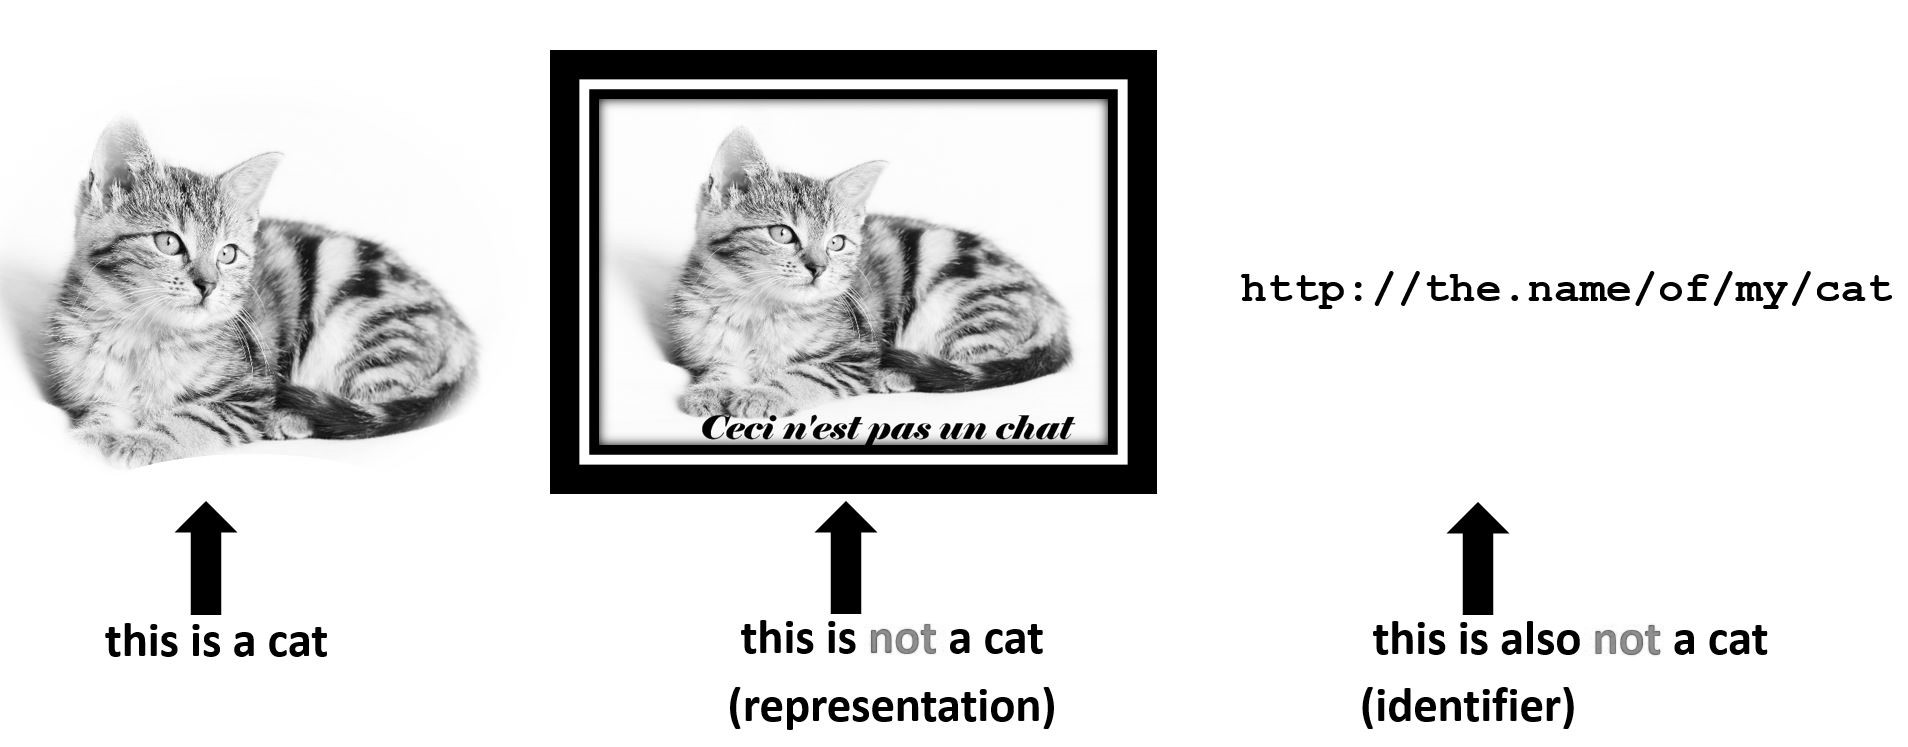
\includegraphics[width=5in]{media/ch5/WebAndCats.jpg}
    \caption{The difference between a cat, a picture of a cat, and an identifier for that cat.  Good linked data practice is to use an identifer that can be used to look up the picture. }
    % free for commercial use, see https://pixabay.com/en/cat-pet-striped-kitten-young-1192026/
    \label{fig:ch5.cats}
\end{figure}

\hypertarget{dereferencing-http-uri}{%
\subsection{Dereferencing HTTP URI }\label{dereferencing-http-uri}}

An HTTP URI is a URI created to name anything we want to talk about 
that  uses  HTTP   as its dereferencing mechanism. When a person or a
software agent (e.g. a Web crawler) comes across that URI, they can easily learn more
about the resource it represents,  by simply making an HTTP call
to the address it provides.   Dereferencing of HTTP URIs is a cornerstone of the hypertext web, and has
functioned well since the beginning of the Web. HTTP URIs come with an
obvious way to get a description about the resource they identify: the
HTTP protocol that can be used to looked them up. Other URI schemes
(e.g. URN, DOI, etc.) require additional services or practices to be
dereferenced.  

We don't use the term URL (Uniform Resource \textbf{Locator}) for these identifiers, to emphasize the 
point that the thing  being
represented may not itself be on the Web at this address, or even at on the Web at all. For example, I
may want to specify an HTTP URI for my cat, Mytsie. No matter how hard I
try, Mytsie herself will never be located on the Web, so I cannot give
her a URL \emph{per se}. But this adorable cat can be identified on the
Web by an HTTP URI, and if you ever go to that address you will be
provided with a description (maybe even a photo or two) on the Web about the resource represented by
that URI, i.e.  Mytsie.

This approach to linked data, in which we use an HTTP URI as an identifier, and 
rely on HTTP-based dereferencing of that URI to provide more information about the resource, 
is summarized in a web design pattern called \emph{Follow Your Nose} \cite{dodds2012linked}. .
According to the  Follow Your Nose pattern,  it is the responsibility of the data publisher
to make sure that the HTTP URIs indeed resolve to web resources that provide
appropriate information. Just as Ariadne provided Theseus a thread to let him
find his way back out of the labyrinth, the web publisher provides HTTP URIs
that allow data consumers to find their way back to the data source, to
learn more about it.  It is up to the data consumer and the details of their application (including issues around performance, trust, scalability,
quality, etc.)
whether they want to follow these links at any particular time. 

%%%%

%Since HTTP URIs rely on the domain names to create the first part of the
%URI scheme, they support the decentralized creation of globally unique
%identifiers. Any owner of a web domain can create and control the access to
%any HTTP URIs in that domain. 

%In choosing and using HTTP URIs, there are
%three important standard mechanisms of the Web and Internet to be aware
%of: the Domain Name Service (DNS) and its implication on the choice of
%domain part of the URIs; content negotiation in HTTP, which allows a
%server to serve different contents for the same HTTP URI to different
%clients; and HTTP redirection, . These three mechanisms and their impacts are
%illustrated in figure~\ref{fig:ch5.2} and detailed in the next sections.

%%%%%


\hypertarget{minting-http-uris}{%
\subsection{Minting HTTP URIs}\label{minting-http-uris}}

How do we choose the URIs we are going to use to talk about the things
we want to describe? What should be their structure or naming schema?
Are there criteria and pitfalls in choosing a method to create URIs for
our collections and applications? These questions are legitimate since
as soon as we start publishing URIs they are reused and referenced and
therefore introduce dependencies and create legacy systems.

The generic form of a URI is describe in their standard
document (URIs are standardized in RFCs from IETF : RFC 3986
  \cite{masinter2005uniform}) like this where values between
square brackets are optional parts one can use in minting a URI (eg.
Indicating a port on a server).

\begin{lstlisting}
scheme:[//[user:password@]host[:port]][/]path[?query][#fragment]
\end{lstlisting}

For instance, a valid URI according to this pattern is for instance:

\begin{lstlisting}
urn:animals.org\#mycat
\end{lstlisting}

As we saw in Section~\ref{usehttp}, using HTTP URIs is the preferred option for the web 
of data, in contrast to other protocols.  An HTTP URI has the form: 


\begin{lstlisting}
http://host[:port]][/]path[?query][#fragment]
\end{lstlisting}


For instance, the following are valid HTTP URIs:

\begin{lstlisting}
http://animals.org#mycat
http://animals.org/cats/mine
http://animals.org/cats/?owner=fabien
...
\end{lstlisting}

The major advantage of using HTTP URIs as identifiers on the  Web  of data is that
they participate in the full infrastructure that drives the hypertext web.  Figure~\ref{fig:ch5.2} shows the three basic mechanism of that infrastructure. 
\begin{itemize}
    \item The \emph{Domain Name Service} (DNS), which associates domain names on the web with internet addresses of web servers,
    \item \emph{Content Negotiation} in HTTP, which allows a web 
     server to serve different content for the same HTTP URI to different
     clients, and
     \item \emph{HTTP Redirection}, which allows a server to redirect a reference
     to another address.
\end{itemize}
The \texttt{host} part of an HTTP URI (\emph{animals.org} in the examples) is managed by 
the DNS (left column of Figure~\ref{fig:ch5.2}).   Someone who wants to publish 
anything on the Web, whether hypertext pages or data, registers a \emph{domain 
name} (e.g., \emph{animals.org}) with the DNS.  Once they have completed this registration, they 
can create and control the access to
any HTTP URIs  that use that domain in the \texttt{host} field. 

The \emph{path} part of the HTTP URI can be arbitrarily long, and is fully at the discretion of
whoever is minting the URL.  This means that there is 
no practical limit on the number of possible URI patterns a data publisher has  at their disposal to name the things they
want to describe on the Web. 

\begin{figure}
    \centering
        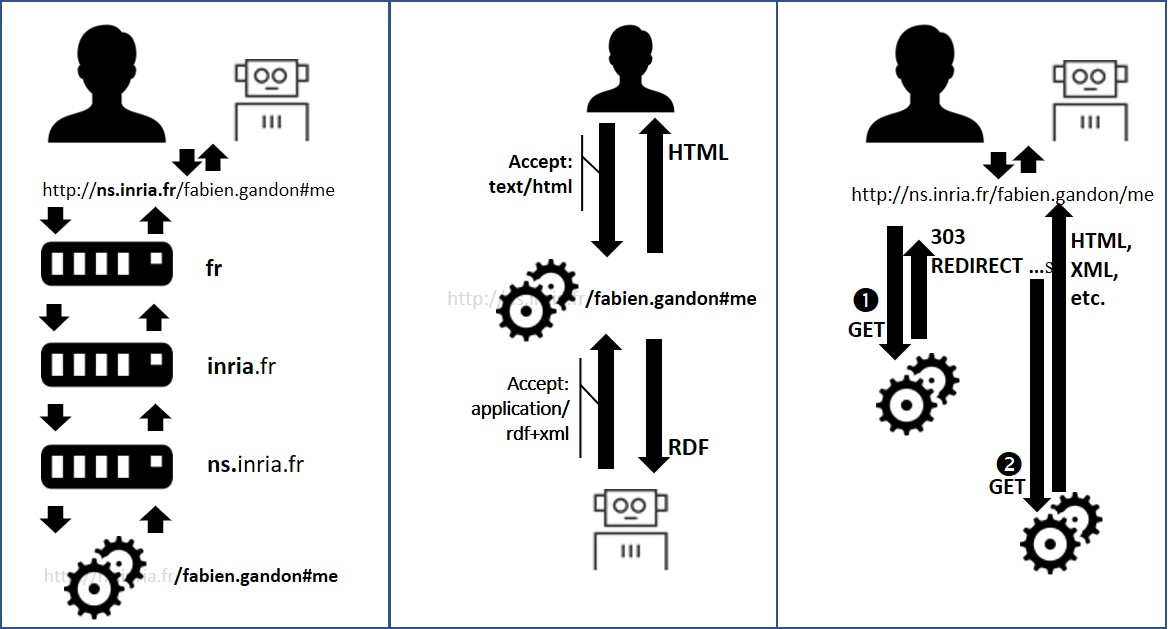
\includegraphics[width=5.0in]{media/ch5/figure-05-02.jpg}
        \begin{tabular}{lll}
        A. Domain Name Service\ \ \ \ \ \ &B. Content Negotiation\ \ \ \ \ &C. HTTP Redirection\ \ \ \  \\
        \end{tabular}
    \caption{Three standard mechanisms used in Web Data publishing and
access}
    \label{fig:ch5.2}
\end{figure}

\subsection{How to build a URI}

Since we are using HTTP URIs for all our data elements, we need to have some 
method for generating enough distinct URIs for everything we want to describe in our data, now and in the future.
The problem of coming up with appropriate identifiers in a large data set is not 
specific to the Semantic Web, and there is no perfect answer. In the context of HTTP URIs for the Semantic Web,
Pros
and Cons have been discussed in several places (
  \cite{Cooluris},
  \cite{URIDoc}).  We will
summarize here some of the things to consider when minting your HTTP
URIs. 


Inspired by the title of an article by Tim Berners-Lee, \emph{Cool URIs don't change}, \cite{dontchange}, a popular proposal for 
minting URIs for the semantic Web is called \emph{Cool URIs}

As suggested by the eponymous article, a key aspect of cool URIs is that they don't change: you want to ensure
that your URIs will be as stable as possible by choosing a stable URI pattern. 
Why is it important to have stable URIs?  
While the ``404 page not found'' error is disappointing on the hypertext web, it can be catastrophic in the Web of Data, where the URIs are the
linkage points between data sets.  A broken link can mean loss of access to an entire data set.

The Cool URI proposal has some advice for how to make URIs stable:

\begin{itemize}
    \item Desing URIs with reference to as few implementation details as possible. In particular, avoid language dependent extensions (.PHP, .json, .rdf), specific server names "desktop8.inria.fr", specific software (\ldots{}/wordpress/\ldots{}), server port number, etc.  
    \item Web servers are able to negotiate content based on information from web clients. Use this feature to avoid implementation details in URIs.
    \item Leave out version information from stable URIs.  The semantic web standards provide ways to specify the version of a data or metadata set, other than changing URIs. 
    \item in many cases, the original data source has some kind of identifier already (a primary key, or an account number, etc.).  You can make use of these to ensure that your URIs correspond to the right data elements. 
\end{itemize}



For example, imagine  we have a table of animals (e.g. a CSV file) with columns
providing information about the vaccination records for our pets, as shown in Table~\ref{tab:ch5.pets}

\begin{table}
    \centering
    \begin{tabular}{|l l l l|}
    \hline
    ID&Species&Name&Expiration Date \\
    \hline\hline
366863&dog&Fido&2020 \\
851903&dog&Bastian&2021 \\
775304&cat&Mytsie&2019 \\
898202&cat&Corvus&2021 \\
847823&cat&Fenris&2019 \\
399378&dog&Maddie&2022 \\
911236&cat&Twinkie&2016 \\
897991&dog&Champ&2019 \\
032579&dog&Zeke&2020 \\
31450&cat&Lila&2019 \\
87580&dog&Fido&2021 \\
\hline
    \end{tabular}
    \caption{Sample data about the vaccine records for our pets. }
    \label{tab:ch5.pets}
\end{table}


The data about the Pet's name and the expiration date of the vaccine cannot be counted on to be  unique
(in this short sample, we have two dogs named Fido).  One option for minting URIs for this would be to include all the data in each URI, as in Table~\ref{tab:ch5.all}.

This method is guaranteed to ensure uniqueness in the data, but makes for very long URIs, and can be misleading if any of the data changes.  Should we coin new URIs?  Or re-use the old ones, which will then reflect out-of-date data?

\begin{table}
    \centering
    \begin{tabular}{|l|}
    \hline
    URI \\
    \hline\hline
http://www.example.com/vac/366863/dog/Fido/2020 \\
http://www.example.com/vac/851903/dog/Bastian/2021 \\
http://www.example.com/vac/775304/cat/Mytsie/2019 \\
http://www.example.com/vac/898202/cat/Corvus/2021 \\
http://www.example.com/vac/847823/cat/Fenris/2019 \\
http://www.example.com/vac/399378/dog/Maddie/2022 \\
http://www.example.com/vac/911236/cat/Twinkie/2016 \\
http://www.example.com/vac/897991/dog/Champ/2019 \\
http://www.example.com/vac/032579/dog/Zeke/2020 \\
http://www.example.com/vac/31450/cat/Lila/2019 \\
http://www.example.com/vac/87580/dog/Fido/2021 \\
\hline
    \end{tabular}
    \caption{Coining URIs by repeating all the data }
    \label{tab:ch5.all}
\end{table}

Since the original data includes an \textbf{ID} field, we can rest assured that this 
will uniquely identify a vaccination, so we can use it for the URI, as in Table~\ref{tab:ch5.id}

\begin{table}
    \centering
    \begin{tabular}{|l |}
    \hline
    URI \\
    \hline\hline
http://www.example.com/vac/366863 \\
http://www.example.com/vac/851903 \\
http://www.example.com/vac/775304 \\
http://www.example.com/vac/898202 \\
http://www.example.com/vac/847823 \\
http://www.example.com/vac/399378 \\
http://www.example.com/vac/911236 \\
http://www.example.com/vac/897991 \\
http://www.example.com/vac/032579 \\
http://www.example.com/vac/31450 \\
http://www.example.com/vac/87580 \\
\hline
    \end{tabular}
    \caption{Coining URIs using the ID field }
    \label{tab:ch5.id}
\end{table}


In order for this method to work, we have to make sure that the column we use really is a unique  identifier. 
For example, we might be tempted to use the column \texttt{name} to coin our URIs.  
This will cause two problems: 

\begin{itemize}
    \item we will end up coining 
\texttt{http://www.example.com/vac/Fido} twice, which will not correctly reflect the data. 
\item Even if there is no  name duplication in our data, one of the animals (say, Mytsie) might be adopted and given a new name (``Missy'').  If this happens, do we have to create a new URI?   Or do we say that the URI at \texttt{<http://example.com/vac/Mytsie>} now has name ``Missy''?
\end{itemize}

In Chapter~\ref{ch3}, we saw how URIs can be abbreviated using namespaces and CURIEs (Compact URIs). 
If we define the prefix \texttt{vac} to be the namespace
\texttt{http://www.example.org/vac/}, then the CURIE for Mytsie's vaccination would evidently   be
\texttt{vac:775304}.   However, there is a constraint on CURIEs \cite{Bray:08:EML} that says that the name after the 
 prefix cannot start with a digit (1, 2,
3\ldots{}) or with basic combining characters (e.g. a comma).  So the proposed CURIE \texttt{vac:775304} is not valid.  Since CURIEs are useful in many contexts, it is good practice to append an alphabetic character at the beginning of the identifier.  So instead of using the URIs in Table~\ref{tab:ch5.id}, we use URIs like those in Table~\ref{tab:ch5.vac}

\begin{table}
    \centering
    \begin{tabular}{|l l|}
    \hline
    URI&CURIE \\
    \hline\hline
http://www.example.com/vac/V366863&vac:V366863 \\
http://www.example.com/vac/V851903&vac:V851903 \\
http://www.example.com/vac/V775304&vac:V775304 \\
http://www.example.com/vac/V898202&vac:V898202 \\
http://www.example.com/vac/V847823&vac:V847823 \\
http://www.example.com/vac/V399378&vac:V399378 \\
http://www.example.com/vac/V911236&vac:V911236 \\
http://www.example.com/vac/V897991&vac:V897991 \\
http://www.example.com/vac/V032579&vac:V032579 \\
http://www.example.com/vac/V31450&vac:V31450 \\
http://www.example.com/vac/V87580&vac:V87580 \\
\hline
    \end{tabular}
    \caption{Coining URIs using the ID field, with an alphabetic character ("V") pre-pended to each numeric ID }
    \label{tab:ch5.vac}
\end{table}

\subsection{Minting URIs in the Wild}
Let us examine two real examples of minting URIs, IETF RFC's and DOIs. 

\subsubsection{URIs for the IETF}
The Internet Engineering Task Force (IETF) is an open
standards organization in charge of developing and promoting the
Internet standards. We have already seen   one of these standards: the URI itself.  It is the IETF who manages registrations for the DNS and the format for URIs.
An official publication of the IETF is   called a \emph{Request
for Comments} (RFC). For instance, the latest RFC that gives the standard specification for
URIs is
\emph{RFC 3986}, which has the title  \emph{Uniform Resource Identifier (URI): Generic Syntax}.
In order to publish the RFCs and support stable references to these
standards, IETF has adopted several URI minting schemes. For instance,
the default URL for an HTML version of an RFC is obtained by concatenating the
domain address \texttt{https://tools.ietf.org/html/rfc} and the RFC number. So, for RFC 3986, we have:

\begin{lstlisting}
https://tools.ietf.org/html/rfc3986
\end{lstlisting}


You can access other versions of the same RFC in plain text and PDF by applying
similar  minting schemes.

For the text version of RFC 3986:
\begin{lstlisting}
https://tools.ietf.org/rfc/rfc3986
\end{lstlisting}

For the PDF version of RFC 3986:
\begin{lstlisting}
https://tools.ietf.org/pdf/rfc3986
\end{lstlisting}

These schemes have the advantage that they are stable; we can use the same URI
for the HTML presentation of the latest RFC version, even as new versions are published.  It has the disadvantage that I cannot refer to RDF 3968 itself, only to particular documents about it.  This violates one of our guidelines for URI formation, that a URI should not include implementation-specific information about a document. We'll see later in this chapter how to use Content Negotiation to address this issue. 

These schemes follow the CURIE suggestion that the final part of the URI begin with an alphabetic character (in this case, it is always 'r'), but they suffer from the drawback that each of them will have a different prefix, since they don't share a common prefix.  If we were to make these into CURIEs, we woud need a separate prefix for \texttt{https://tools.ietf.org/rfc/}, \texttt{https://tools.ietf.org/pdf/} and  \texttt{https://tools.ietf.org/txt/}. 

\subsubsection{URIs for ISO DOIs}


As a second example, we can consider a family of identifiers
standardized by 
The International Organization for Standardization (ISO) maintains a standard family 
of identifiers (ISO~26324) to uniquely identify objects including books, articles, data sets,
videos, etc. This family of identifiers is called \emph{digital object
identifier} (DOI) and is used to identify and reference digital
resources in a sustainable manner. For instance, ISO assigned to the article entitled
``Distributed Artificial Intelligence for Distributed Corporate
Knowledge Management'' published by Springer the DOI

\begin{lstlisting}
doi:10.1007/3-540-45741-0_18
\end{lstlisting}


The ISO  provides an online service that looks up any DOI and provides a corresponding HTTP
URI.   For example, the service (available at https://www.doi.org/) translates this DOI into the HTTP URI:


\begin{lstlisting}
http://doi.org/10.1007/3-540-45741-0_18
\end{lstlisting}


This HTTP URI will then redirect you to a description of the object
identified by the DOI.  

The advantage of these URIs is that they are stable; ISO makes sure that for a particular 
resource, the DOI will not change.  They have the drawback that they cannot be formed into 
CURIEs, since the final component begins with a number. 




%Once you have established a pattern for  URIs, we will see in the next
%sections that HTTP content negotiation (also called \textit{conneg}) and,
%ossibly, \textit{redirections} have to be configured on the server to provide
%content in XML, RDF, HTML, JSON, etc. to whomever looks up these URIs.
%But before we move to these next steps, let us look at the implications
%of the choice of a domain name for your URIs.


\section{HTTP and the Architecture of the web}

Figure~\ref{fig:ch5.2} shows the basics of the architecture of the web as three pillars; the domain name service, content negotiation, and redirection.  We now take a deep dive into how this architecture influences the way we as  publishers and consumers of data interact with the Web of data. 

\hypertarget{king-of-my-domain}{%
\subsection{Ruler of My Domain}\label{king-of-my-domain}}

We'll start with Domain Name Resolution, or DNS for short  figure~\ref{fig:ch5.2}(A). 

The first step in resolving an HTTP URI is to identify what host (machine) on the internet 
to query get data about the resource identified by the URI. HTTP URIs rely on the Domain Name System (DNS) for this function.
The DNS is a decentralized hierarchical naming system for identifying
devices and services connected to the
Internet. Anyone who browses the Web use the DNS every day, because it provides the service that
transforms a domain name (e.g. ns.inria.fr)
into the internet address (IP address e.g. 128.93.162.87) of the machine
or service in charge of answering for that domain.  Although the host
machine could be identified in the HTTP URIs by its IP address directly
(e.g. http:// 128.93.162.87/ is a valid HTTP URI), there are two advantages to 
using a name service to provide domain names instead of IP addresses.  First, we humans prefer
domain names that are easier to read and memorize (e.g.
http://ns.inria.fr).   More importantly for a stable web of data, the use of domain names 
provide stable URIs, allowing a data provider to change a server's
addresses without changing the URIs of the data that is hosted there.

%This mechanism allows us to agree
%on the way we name things but it does not prevent peoples to mint
%different names for the same purpose or to disagree on the descriptions
%of the things they identify. We will not all agree on what the thing
%means, but 

In the context of dereferenceable HTTP URIs, the DNS
makes sure that if anyone in the world resolves a particular HTTP URI, they
will all get to the same place.   This provides us a world-wide reference mechanism.  We 
might not want to say the same things about Mytsie the cat 
(e.g., I might want to say that she 
is calico, and another source might want to record her weight from week to week).  
Different sources might even disagree; someone else might claim that she is tortoiseshell, 
not calico.  In a world-wide distributed web of data, we can't expect everyone to agree on 
their statements
about Mytsie, but the DNS provides a mechanism so we can agree on which thing we are 
disagreeing about.

Now that we understand how DNS works and its importance in HTTP URs, what does this mean
for choosing URIs for our data? Since any look up on a URI starts with  domain name 
resolution, whoever controls the DNS registraion for a
domain name controls the access to the HTTP URIs minted with that domain
name, in the sense that they can specify what server the DNS will map the URIs to. 
So if you lose control over a domain name you lose control of the
linked data using that domain in there URIs, in the sense that you no
longer control the answer provided when the HTTP URIs are dereferenced
and accessed.

Therefore, one must be careful in choosing the domain name for the \texttt{host}
part of a URI pattern one uses as identifiers in publishing linked data
because it is key to ensure persistence and control of dereferenceable
URIs.  In Chapter~\ref{ch3}, we saw some namespaces that have been defined 
by the World Wide Web consortium (the W3C) themselves, to define namespaces for 
\texttt{rdf:}, \texttt{rdfs:} and \texttt{owl:}. Now we understand more deeply what this
means. If you want to look up what any resource in one of these namespaces means, 
for example, \texttt{rdf:type} 
(short for \texttt{http://www.w3.org/1999/02/22-rdf-syntax-ns\#type}, you can 
find it by resolving that URI (try it in a web browser!).  The result is controlled by the 
W3C, becasue the W3C owns the domain at w3.org. 


We have already seen several standard namespaces from the W3C, and in the following 
chapters, we will see some more.  In each case, the W3C publishes a namespace along 
with information about the resources in that namespace.  All of these namespaces have HTTP 
URIs using the domain  \texttt{w3.org} as the host, ensuring that when anyone looks 
them up they get the answer that the W3C chose to provide.  What we will now see is
that each of the access to this service can negotiate a customized
answer.

\hypertarget{negotiating-your-web}{%
\subsection{Negotiating your Web}\label{negotiating-your-web}}

The second pillar of the Web architecture shown in Figure~\ref{fig:ch5.2} is  Content Negotiation.

So far, we have been talking primarily about a Web of Data.  But in fact, there  is only one
Web with all its different facets interlinked, including data, hypertext, schemas,
services, etc.  The Web is intended to be used at the same time by
machines and by humans as a shared common space for hybrid communities
of natural intelligence and computational intelligence. Therefore, a
human user or a software agent must both be capable of obtaining
descriptions of any particular resource described on the Web  in the most suitable
format for them, for example,  a Web page in HTML for a human reader  and an RDF/XML
description for a Web robot.   Furthermore, each human will have some preferences (e.g.
in terms of which human language they prefer, e.g.,  English, Chinese or French) and
software may have specific preferences as well  in terms of the format an application may prefer (e.g., 
data in JSON-LD vs. CSV).

Using the HTTP protocol (\cite{leach1999hypertext}), a Web client
can negotiate the content of a response to an HTTP URI look up: whether
you are interested in a Web of hypertext because your application is
displaying the results directly to humans or you are interested in a data packet 
because your application is linking together the Web of data, 
the content negotiation mechanism of HTTP
allows you to state the form of content that is most suitable to you.

The Content Negotiation mechanism, sometime called \emph{conneg} for short, is part of the
HTTP standard. The HTTP protocol allows Web clients to set headers in
the requests they send in order to specify their preferences in
particular in terms of format. These headers rely on several standards
to allow you to specify formats (media types or MIME types \cite{klensin2013media}), 
natural languages (ISO
language codes \cite{iso_language_639}), etc.

Using these preferences, the server may decide to adapt its response or
re-route the request to best serve the client. It is the responsibility
of the server to match between the preferences of the client and the
options it has available, and to select the best response for the
client. As a result, as shown in Figure~\ref{fig:ch5.2}B,  the same URI may be accessed
by two different clients: the client used by humans (e.g. a Web browser)
could retrieve an HTML description while a software  application could
negotiate an RDF description at the very same HTTP URI.

Going even further, the HTTP content negotiation can be used by linked
data applications to negotiate the RDF syntax they prefer (e.g. XML,
Turtle, JSON-LD, see Chapter~\ref{ch3}) or alternate representations for their interfaces (e.g.
HTML, text, image, etc.).

Let us give an example, this time from the DBpedia site providing RDF
data extracted from Wikipedia. There, the thing \emph{Paris} is identified
by

\begin{lstlisting}
http://dbpedia.org/resource/Paris
\end{lstlisting}

If you lookup that URI as a human in a Web browser (try it), content
negotiation will redirect you to a Web page for humans:

\begin{lstlisting}
http://dbpedia.org/page/Paris
\end{lstlisting}

But if you are an application you can negotiate data and land at the
address:

\begin{lstlisting}
http://dbpedia.org/data/Paris
\end{lstlisting}

the result is a data set expressed in RDF (by default, in RDF/XML).  

In this way, \emph{conneg} allows us some flexibilty in the use of HTTP URIs;  we can use 
the same URI for the hypertext Web and the data Web (which, after all, are the same Web), but
provide different responses depending on who is doing the asking.  It is, of course, the server's responsibility to make sure that the content of the response is the same, regardless of its form. 

%% finish this sentence!! - FG, please review the previous paragraph.  
%% In the original, the text simply ended, so I finished what I thought 
%% you had in  mind here. 

\hypertarget{rerouting-calls}{%
\subsection{Rerouting calls}\label{rerouting-calls}}

The final pillar of Figure~\ref{fig:ch5.2} is  \emph{HTTP redirection}.

Anyone who has ever browsed the web is familiar with the ``404 Not Found'' error we sometime 
get in our browser
when accessing a link that is broken because the URL no longer exists
(e.g. the page was deleted) or never existed (e.g. we misspelled the
URL). The code 404 is one of the most well-known error code of HTTP
because it is the one we are the most likely to see. However there are
many other codes such as the ``200 OK'' that we get all the time but we
don't see because it means the HTTP request was successful and the
response provides the content or result we were asking. The mundane use
of the HTTP redirection mechanism is to avoid broken links: when a page
is moved, when a Web application is redesigned or when a Web site is
relocated, and HTTP redirection may be set up on the Web server to
redirect Web clients to the new address where a content or service has
moved. When you browse the Web this happens all the time and you won't
even notice it unless you pay attention at the changes in the address
bar of your Web browser. Redirection may use several codes all starting
with the digit 3 and characterizing the type of the redirection, for
instance the code 301 means the requested resource has been assigned a
new permanent URI given in the answer while 302 means it resides
temporarily under a different URI provided in the answer.

When using HTTP URIs to identify resources that are not on the Web
themselves (eg. a cat, a car, a law, a person, etc.) it would not be
appropriate to respond ``200 OK'' since the identified resource cannot
be accessed via the Web. Using ``404 Not Found'' would also be
misleading because it would mean the URI is not recognized.

One possibility is to use the HTTP code ``303 See Other'' which is a way
to reroute the request to another address where a response can be found.
The 303 response looks like this, with the location header specifying
the other address to lookup:

\begin{lstlisting}
HTTP/1.1 303 See Other

Location: http://animals.org/page/cat/1278
\end{lstlisting}


In our case responding 303 to an HTTP URI means that the service that the DNS 
referred the URI to is unable to provide a representation of the target resource, but
it can refer the requester to another resource instead, which 
is also description of the target resource, and which can be
transferred over HTTP. The 303 code provides us a Web-compatible way of
responding to a request for a URI that identifies a things that are not
on the Web.

The description to which the requester is redirected must contain
information about the target resource. If the negotiated content is a
Web page, at least some content of that page must be about the targeted
resources. If the negotiated content is RDF, at least some triples of
the answer must use the URI of the target resource.

\hypertarget{hash-or-slash}{%
\section{Hash or Slash}\label{hash-or-slash}}

Even inside the last parts of the URIs (path, query and
fragment) there are minting choices that impact the performance in
dereferencing a URI. In particular, if you intend to support
dereferenceable HTTP URIs, there are two main design patterns you can 
considered when you want to choose a naming scheme to identify
things that are not on the Web. These two families are referred to as
the ``hash URIs'' and the ``slash URIs''.  

%These two options were the subject of many discussions we will not detail here.

If the reader is familiar with the book ``Gulliver's Travels'' and its
influence on computer science, at first this distinction can sound like
a debate between little-endian and big-endian. However these are the two
main ways to support the provision of a description of the identified
things respecting the HTTP semantics and keeping different URIs for the
things and their descriptions. Both ways can be coupled with content
negotiation to serve the most appropriate format. Let us now see each
option in more details and their advantages and disadvantages.

In the option called ``hash URIs'' the URI contains the hash character
("\#") which is the technical mark of a fragment identifier inside the
URI ; the fragment identifier is the \# and the string that follows it.
In a URL it is traditionally used to denote a fragment of a Web page
e.g.

\begin{lstlisting}
http://fabien.info/publications.html#navothers
\end{lstlisting}

This could indicate a section ``navothers'' in the page
``publications.html''

When a hash (\#) separates a fragment in a URI to be looked up, the
dereferencing consists in removing that fragment and accessing the
source by performing a look up on the URI before the fragment. Following
our example, a Web browser would only access:

\begin{lstlisting}
http://fabien.info/publications.html
\end{lstlisting}

Then, with the representation it retrieved, the Web browser can reuse
the provided fragment, for instance to automatically scroll down to the
section it identifies in the document.

Generalizing this example, whenever a URI contains a hash (\#), this
indicates a fragment in the URI:

\begin{lstlisting}
http://my.domain.name/my/path#the-fragment
\end{lstlisting}


And because the HTTP standard requires the Web client to remove the
fragment before making a request if you make an HTTP call on this URI
your client will in fact perform it on the address:

\begin{lstlisting}
http://my.domain.name/my/path
\end{lstlisting}


Using fragments in HTTP URIS, the URI of the thing (with the fragment)
and the URI of the description (without the fragment) are two different
identifiers.

The use of a fragment has two advantages:

\begin{enumerate}
\def\labelenumi{\arabic{enumi}.}
\item
  it differentiates between the name of the descriptions and the
  names of the resources described without performing a redirection, and
\item
  it allows grouping of several descriptions in a single resource that can be
  cached by a client to avoid several calls to discover different linked resources.
\end{enumerate}

For example, in one source at the address:

\begin{lstlisting}
http://workingontologist.org/fabien/objects/cars
\end{lstlisting}


I can describe several things:


\begin{lstlisting}
http://workingontologist.org/fabien/objects/cars#bmw1
http://workingontologist.org/fabien/objects/cars#smart1
http://workingontologist.org/fabien/objects/cars#tesla1
\end{lstlisting}
\ldots{} 

These advantages of hash URIs can also be a drawback; since the whole
description source is retrieved every time the address is accessed, one
cannot obtain the description of just a  single resource.  This could 
be costly in terms of network traffic, memory and processing
when the set of described resources is large.

The alternative is to use only slash URIs (i.e. the symbol /) 
to generate identifiers. For instance:

\begin{lstlisting}
http://workingontologist.org/fabien/objects/cars/bmw1
\end{lstlisting}


This is the second option called ``303 URIs'' or ``slash URIs'' or ``303
redirect'' that relies on the use of the "303 See Other" HTTP answer to
redirect accesses to the HTTP URI of a thing to some URL where to find a
description about that thing.

The dereferencing of an HTTP Slash URI identifying a thing follows  a four-step 
process in four steps: 
\begin{enumerate}
    \item The client makes the first
attempt to connect (HTTP GET) to the HTTP Slash URI; 
    \item the server
respond with a ``303 See Other'' HTTP code and provides the URL to get a
description;
    \item the client performs a second call (HTTP GET) to the
provided URL;
    \item the server provides the requested description (200
OK).
\end{enumerate}

Just as is the case for any URI resolution, yhis process can be combined with 
content negotiation so that
the result provided by the web server corresponds as closely as possible to the preferences
of the client.

The slash URI alternative allows us to be much more modular in
the storage and transfer of descriptions. In this case, a Web client can
retrieve only the description it is interested in.

Disadvantages include the multiplication (by two) of HTTP calls (the
initial access and the second one after the redirection) and the
fragmentation of the data that requires multiple calls when one wants to
retrieve a collection of them.

To summarize, fragments can be used for small data sets where grouping
makes sense (unity of content, linked, same life cycle), a classical
example of that are vocabularies, schemas or ontologies. This option is
also simpler as it can be implemented, for instance, just by
hosting a file on a Web server. The redirection by HTTP 303 is more
technical but allows more control over the data served.

Finally, nothing prevents you from using and mixing these two options
even inside the same data set. A classical way to do that is to add an
artificial fragment (e.g. \#me, \#this) to combine the modularity of 
slash URIs with the simplicity  of  hash URIs. For example, we can have a full
path with slashes to generate identifiers allowing us to be modular in
the storage and transfer of descriptions and add an artificial fragment
(\#this) to enforce that the URI of the thing (with the fragment) and
the URI of the description (without the fragment) are two different
identifiers and avoid a redirection. In this way, we can have our
cake and eat it too:

\begin{lstlisting}
http://workingontologist.org/fabien/objects/cars/tesla1#this
\end{lstlisting}

\hypertarget{see-it-for-yourself}{%
\section{See it for yourself\ldots{}}\label{see-it-for-yourself}}

This chapter is about linked data on the \emph{Web}.  To illustrate 
how this works, we will examine some examples taken directly from the Web. At
the moment of writing this book, most these examples are online and
accessible.   But things change fast on the Web, so there is no guarantee that 
any particular example will work in the future.   We'll provide a number of examples,
in the hopes that at least some of them will continue for a while.  This has the added benefit 
that it allows us to demonstrate a wide range of uses of linked data on the web. 

\subsection{Bibliography at DBLP}

DBLP is a service that manages bibliographic information for publications
in computer science around the world \cite{DBLP:conf/spire/Ley02}.  Each 
publication that is documented in DBLP is also available as data in RDF. 
There is a link on each page to access the RDF data in any of several 
formats.  Keeping with the conventions of this book, we will show the
RDF data in Turtle format, even though that is not one of the download formats 
available directly from DBLP. 

For example, the Second Edition of \emph{Semantic Web for the Working Ontologist} is 
indexed in DBLP, and is given the identification index number 0028543.  Information about
the publication is available both in human-readable HTML form, as shown in Figure~\ref{fig:ch5.3}, 
which is available at the URL \url{https://dblp.org/rec/html/books/daglib/0028543}, and in machine-readable form
in RDF, which is available from the URL \url{https://dblp.org/rec/rdf/books/daglib/0028543}. 
The triples for this part of the data sets are given in Turtle format in Figure~\ref{fig:ch5.4}.


\begin{figure}
    \centering
     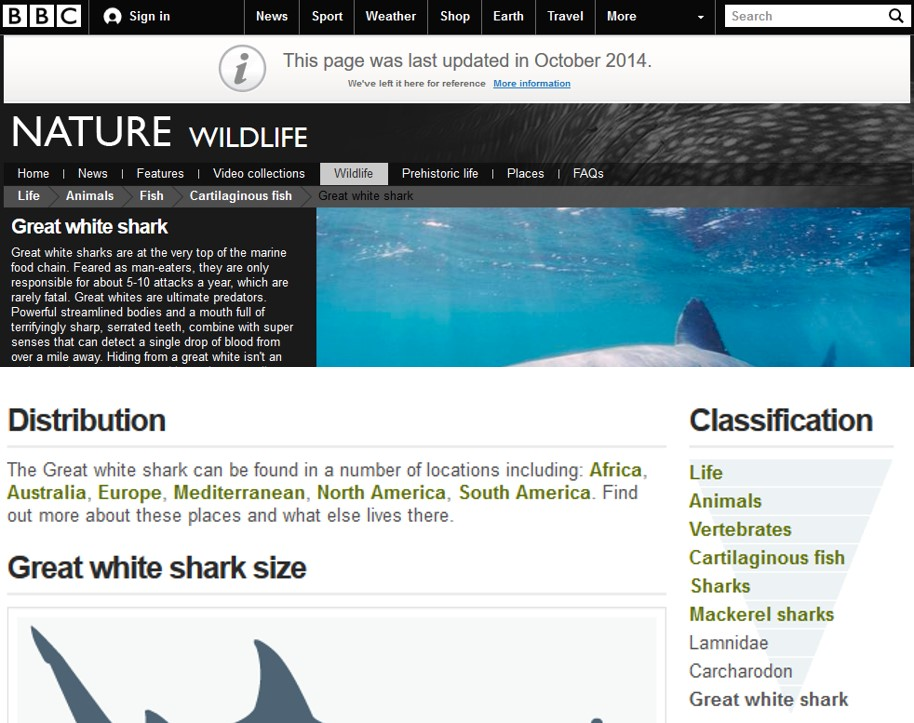
\includegraphics[width=5.0in]{media/ch5/figure-05-03.jpg}
    \caption{HTML rendering for humans of the bibliography for the Second Edition of Semantic Web for the Working Ontologist, from dblp.org}
    \label{fig:ch5.3}
\end{figure}





\begin{lstlisting}
http://www.bbc.co.uk/nature/life/Great_white_shark.rdf
\end{lstlisting}

\begin{figure}
\begin{lstlisting}
<https://dblp.org/rec/books/daglib/0028543>
 rdf:type dblp:Publication ;
 owl:sameAs <urn:isbn:978-0-12-385965-5> ;
 dblp:title "Semantic Web for the Working Ontologist - Effective Modeling in RDFS and OWL, Second Edition." ;
 dblp:bibtexType bibtex:Book ;
 dblp:publicationType dblp:Book ;
 dblp:authoredBy <https://dblp.org/pers/a/Allemang:Dean> ;
 dblp:authoredBy <https://dblp.org/pers/h/Hendler:James_A=> ;
 dblp:primaryElectronicEdition <http://www.elsevierdirect.com/product.jsp?isbn=9780123859655> ;
 dblp:pageNumbers "I-XIII, 1-354" ;
 dblp:yearOfPublication "2011" ;
 dblp:publishedBy "Morgan Kaufmann" ;
 dblp:isbn13 "978-0-12-385965-5" .
\end{lstlisting}
    \caption{Machine readable version of the bibliography for the Second Edition of Semantic Web for the Working Ontologist, from dblp.org}
    \label{fig:ch5.4}
\end{figure}

DBLP is a simple example of how the same data can be served in different forms for different
purposes; the human-readable HTML is difficult for a machine to read because of typesetting and styling
which make it easier and more attractive for human readers, whereas RDF triples are difficult for
humans to read because of their reliance on cross-referencing and unique identifiers that make them
easier for a machine to process. 

\subsection{Publishing Protein Sequences}

The Universal Protein Resource (\emph{UniProt} for short) is a service whose mission is to 
provide the scientific community 
with a comprehensive, high-quality and freely accessible resource of protein sequence and 
functional information \cite{10.1093/nar/gky1049}. 
Among its services, UniProt  provides RDF descriptions of protein sequence and
function. For example, if you are a biologist interested in the ``Cell surface
glycoprotein MUC18'', there is a URI for that:

\begin{lstlisting}
http://purl.uniprot.org/uniprot/P43121
\end{lstlisting}


\begin{figure}
    \centering
    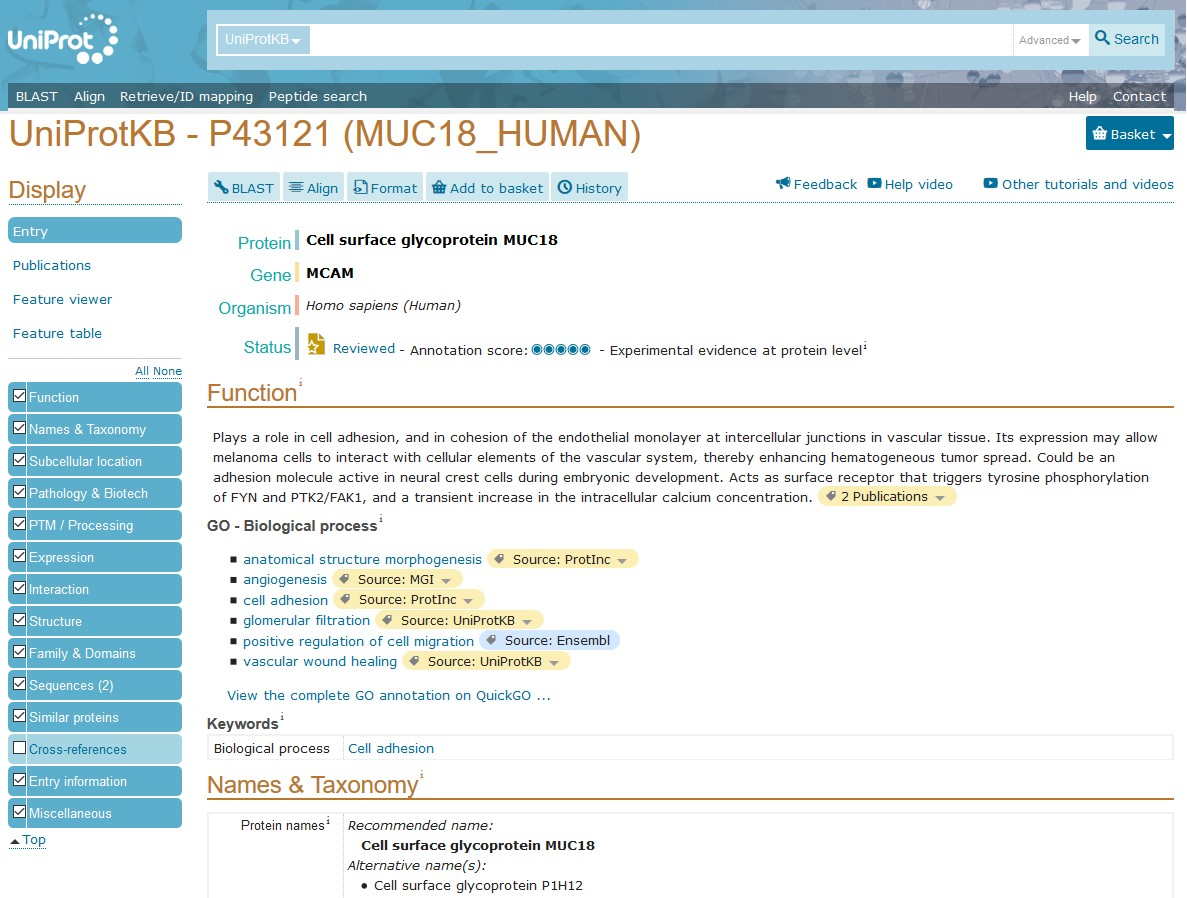
\includegraphics[width=5.0in]{media/ch5/figure-05-05.jpg}
    \caption{Cell surface glycoprotein MUC18 in UnitProt: extract of the HTML
rendering for humans.  From uniprot.org edited only for color, licensed as CC BY 4.0 https://www.uniprot.org/help/license }
    \label{fig:ch5.5}
\end{figure}

UniProt's service provides a good example of URI redirection.  The persistent URI is \texttt{http://purl.uniprot.org/uniprot/P43121}.  
When this HTTP URI is accessed by a Web browser for a human,  the response is a redirection to 

\begin{lstlisting}
https://www.uniprot.org/uniprot/P43121
\end{lstlisting}

which resolves to an HTML
page suitable for display in a browser (see Figure~\ref{fig:ch5.5}).   

On the other hand, when  that same HTTP URI is accessed by a 
machine,  the
response is a redirection to an RDF version of that description:

\begin{lstlisting}
https://www.uniprot.org/uniprot/P43121.ttl
\end{lstlisting}

This redirected URI resolves to an RDF document, an excerpt of which can be seen in 
Figure~\ref{fig:ch5.6}.


\begin{figure}
\begin{lstlisting}
:P43121 rdf:type up:Protein ;
  up:reviewed true ;
  up:created "1995-11-01" ;
  up:modified "2019-05-08" ;
  up:version 173 ;
  up:mnemonic "MUC18_HUMAN" ;
  up:oldMnemonic "MU18_HUMAN" ;
  up:replaces <O95812> ,
    <Q59E86> ,
    <Q6PHR3> ,
    <Q6ZTR2> ;
  up:citation citation:2602381 .
\end{lstlisting}
    \caption{Cell surface glycoprotein MUC18 in UnitProt: extract of the
Turtle version for automated use.  From uniprot.org unedited, licensed as CC BY 4.0 https://www.uniprot.org/help/license}
    \label{fig:ch5.6}
\end{figure}

\subsection{Wikipedia as Data: DBpedia}
\label{dbpedia}

\emph{DBpedia} is a crowd-sourced community effort to extract structured
content from the information created in various Wikimedia projects\cite{Auer:2007:DNW:1785162.1785216}. 
This includes the famous Wikipedia encyclop{\ae}ia.  This initiatives extracts
and publishes structured data from the pages of Wikipedia
and other Wikimedia projects, and therefore covers a wide variety of
domains and topics. As in the other examples in the chapter, DBpedia uses RDF and linked data 
principles in the publication of their information. 
Thus, every topic has an HTTP URI, the description of which, using redirection and \emph{conneg},  
is provided  either as
HTML or as 
RDF. Let's take as an example the concept ``Eiffel Tower'', which is identified by the
following identifier:

\begin{lstlisting}
http://dbpedia.org/resource/Eiffel_Tower
\end{lstlisting}

If you access that HTTP URI with a browser, you are redirected to the
following URL

\begin{lstlisting}
http://dbpedia.org/page/Eiffel_Tower
\end{lstlisting}

This URL displays an HTML page rendering all the data extracted about
that topic and available publicly on the Web as linked data (Figure~\ref{fig:ch5.7}).

\begin{figure}
    \centering
    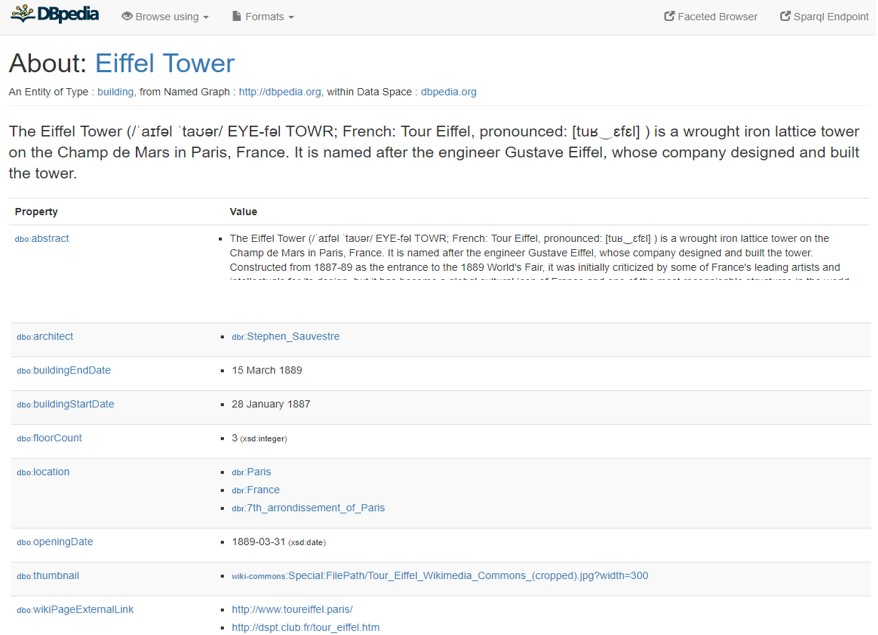
\includegraphics[width=5in]{media/ch5/figure-05-07.jpg}
    \caption{Eiffel Tower at DBpedia: extract of the HTML rendering for humans. From dbpedia.org edited for color only, CC BY SA https://creativecommons.org/licenses/by-sa/3.0/us/}
    \label{fig:ch5.7}
\end{figure}

At the same HTTP URI you can negotiate many other formats including, for
instance RDF using Turtle/N3 syntax. You would then be redirected
(Figure~\ref{fig:ch5.8}) to another URL for instance:

\begin{lstlisting}
http://dbpedia.org/data/Eiffel_Tower.n3
\end{lstlisting}


\begin{figure}
 \begin{lstlisting}
1.	@prefix dbo:	<http://dbpedia.org/ontology/> .
2.	@prefix dbr:	<http://dbpedia.org/resource/> .
3.	@prefix rdf:	<http://www.w3.org/1999/02/22-rdf-syntax-ns#> .
4.	@prefix umbel-rc:	<http://umbel.org/umbel/rc/> .
5.	@prefix dbp:	<http://dbpedia.org/property/>
6.	@prefix wikidata:	<http://www.wikidata.org/entity/> .
7.	dbr:Eiffel_Tower
8.	rdf:type	umbel-rc:Skyscraper, wikidata:Q41176, umbel-rc:Building,
                    dbo:Location, dbo:Place, dbo:Building ;
9.	dbo:buildingStartDate	"28 January 1887" ;
10.	dbp:years	1889 ;
11.	dbo:floorCount	"3"^^xsd:positiveInteger ;
12.	dbp:mainContractor	dbr:Gustave_Eiffel ;
13.	dbo:location	dbr:Paris ,
14.	<http://dbpedia.org/resource/7th_arrondissement_of_Paris> ,
15.	dbr:France ;
16.	dbp:latd	48 ;
17.	dbp:latm	51 ;
18.	dbp:longd	2 ;
19.	dbp:longew	"E"^^rdf:langString ;
20.	dbp:longm	17 ;
21.	dbp:elevatorCount	8 ;
22.	dbp:height	300 .
 \end{lstlisting}
    \caption{Eiffel Tower at DBpedia: extract of the RDF/Turtle version for
machines. From dbpedia.org, edited for format.  CC BY SA https://creativecommons.org/licenses/by-sa/3.0/us/}
    \label{fig:ch5.8}
\end{figure}

Now let us fully play the game of linked data. In (Figure~\ref{fig:ch5.8}) you can
find a triple (line 8) saying that the Eiffel Tower is of type
wikidata:Q41176 which is a CURIE using the namesace prefix \texttt{wikidata:}, which is defined 
on line 6. At this stage we don't know what this
means, but we can follow our nose by expanding the CURIE (i.e., 
replacing the prefix with its defined  namespace) to obtain an HTTP URI that we
can access:

\begin{lstlisting}
http://www.wikidata.org/entity/Q41176
\end{lstlisting}

If you access that HTTP URI with a browser, you are redirected to the
following URL

\begin{lstlisting}
https://www.wikidata.org/wiki/Q41176
\end{lstlisting}


This URL resolves to an HTML page that displays all the data about this
resource.   
(Figure~\ref{fig:ch5.9}). This page is part of another important  data source on the Web of data, 
\emph{Wikidata}. Wikidata is  is another initiative of the Wikimedia Foundation, which provides 
central storage for the structured data used in other projects of the
foundation,  including Wikipedia, Wikivoyage, etc.  Like many of the initiatives of the Wikimedia foundation, this knowledge
base is open on the Web and can be read and edited by both humans and
machines.

\begin{figure}
    \centering
    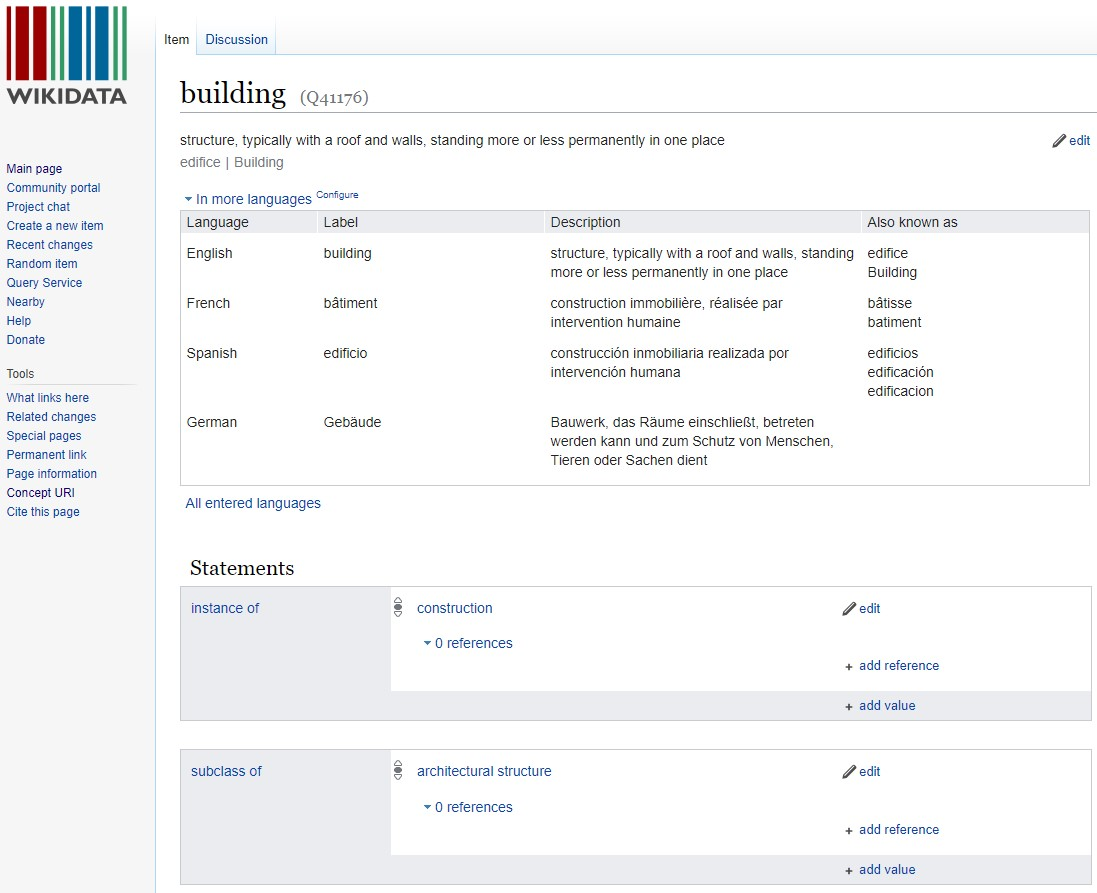
\includegraphics[width=5.0in]{media/ch5/figure-05-09.jpg}
    \caption{``Building'' at Wikidata: extract of the HTML rendering for humans.}
    \label{fig:ch5.9}
\end{figure}

As we have seen in the other examples, an application can specify that it prefers  another format for 
the same data (Figure~\ref{fig:ch5.10}), for
instance,  as  RDF N-Triples (see Section~\ref{ntriples}).  

Putting  all the pieces
together, we can see that this mysterious resource called \texttt{wikidata:Q41176},
which  was found among the types of the Eiffel Tower listed in DBpedia, represents the
category of \texttt{Buildings} as represented in  Wikidata.   
In order to get the big picture of the Eiffel Tower, 
including the fact that it is a building, we combine information from two data sets: DBpedia and Wikidata. 
In this way, we have
witnessed a link across two data sources on the Web of data.

\begin{figure}
 \begin{lstlisting}
<http://www.wikidata.org/entity/Q41176> rdfs:label "building"@en .
<http://www.wikidata.org/entity/Q41176> skos:prefLabel "building"@en .
<http://www.wikidata.org/entity/Q41176> <http://schema.org/name> "building"@en .
<http://www.wikidata.org/entity/Q41176> rdfs:label "Bilding"@pih .
<http://www.wikidata.org/entity/Q41176> skos:prefLabel "Bilding"@pih .
<http://www.wikidata.org/entity/Q41176> <http://schema.org/name> "Bilding"@pih .
<http://www.wikidata.org/entity/Q41176> rdfs:label "budova"@sk .
<http://www.wikidata.org/entity/Q41176> skos:prefLabel "budova"@sk .
\end{lstlisting}
    \caption{Building at Wikidata: extract of the RDF N-Triple version for
machines}
    \label{fig:ch5.10}
\end{figure}




\hypertarget{linking-rdf-data}{%
\subsection{Linking RDF data}\label{linking-rdf-data}}

The recommended format for publishing linked data on the Web is RDF,  and as we saw in Chapter~\ref{ch3}, it 
has different serialization formats (XML, Turtle,
JSON-LD, RDFa, etc.).  These formats can be specified as   part of the content negotiation when
dereferencing an HTTP URI.   But regardless of the serialization, the content is given as 
a set of triples (Section \ref{distribute}), where each component of each triple is an HTTP URI. 

The very fact that RDF relies on URIs to identify
everything makes it an excellent data model for publishing,
exchanging and extending descriptions on the Web. The use of HTTP URIs
provides a standard way to obtain and augment data about any 
identifier. In fact, an RDF triple contains up to three HTTP URIs
(subject, predicate and object), and each can be used to follow our
noses and discover new data. Any HTTP URI used in an RDF data set
can be looked up for more information.

In this sense,   any RDF data set already contains links, since
RDF triples are links between one resource and another.  
But this sense of linkage isn't enough to weave a Web of data.  After all, 
If each data source were to only use  URIs from  its own domain, then
that source would be an isolated island,  and there would be no
Web of data.  To
weave a Web of linked data we need links across data sets,  which means the
subjects or objects of the triples of one data set have to reuse
URIs from some other data sets.  As a good practice, the more such links, the better, 
since it means we have a more densely interconnected web of data, which in turn, supports
improved discovery,  crawling, integration, browsing,
aggregation, etc. of multiple data sources

External links can be established in many different ways.
\begin{enumerate}
    \item A new data set can create its own URIs for common entities.  This is 
    the most likely scenario for data sets that have been created on their own, without
    expectation that they will be part of a Web of data.  In this case, links
    are established later on by identifying the fact that some URI in the new data sets
    actually refers to an entity that already has a URI in another data set.  
    
    \item{A designer of a new data set can make an effort to re-use URIs that have already been established by 
    existing data sets.  This method requires a bit more effort up front, since the designer of the new 
    data set has to determine which URI corresponds to the thing they are describing. This up-front 
    work can pay off in the long run,  since
    there is no need to establish later on whether two entities really are intended to refer to the same thing. 
    In this case, the data designer has already made that clear.  
    \label{ref}
    }
    
    \item In many cases, a standard is already available for some entities, but it has not been published as 
    linked data.  For example, the ISO publishes short (i.e., up to three character) codes for countries of the world. 
    A variant of the  option \ref{ref} above is to coin a URI using that standard.  The Object Management Group (OMG) publishes Languages, Countries and Codes (LCC) using this strategy (among others).  For example, the URI for the ISO code for Great Britain is 
    \begin{lstlisting}
    http://www.omg.org/spec/LCC/Countries/ISO3166-1-CountryCodes/GB
    \end{lstlisting}
    You don't have to look this up 
    at the OMG; you can build this slash URI yourself, once you know that the ISO 2-digit code for Great Britain is \texttt{GB}. Just append the ISO 2-digit country code at the end of 
    \begin{lstlisting}
    http://www.omg.org/spec/LCC/Countries/ISO3166-1-CountryCodes/
    \end{lstlisting}
    
    \item Another variant of option \ref{ref} above is for a data set to link to a schema.  We will see schema languages for RDF in Chapters \ref{ch8} (RDFS), \ref{ch9} (RDFS-Plus), \ref{ch11} (SKOS) and \ref{ch12} (OWL).  These schema languages typically define metadata entities like \emph{classes} and \emph{properties} that can be used to align data.  These classes and properties themselves are identified by HTTP URIs.   \label{schem}
\end{enumerate}

To elaborate on option \ref{schem}, as far as the URIs are concerned, it is identical to option \ref{ref}. 
but in this case, the URIs refer to class names and property names (which might correspond to table names and field names 
if the data were originally represented in a relational data store).  
When two or more data sets re-use the same schema, it is easier to federate the data sets.  

As an example, the Financial Industry Business Ontology (FIBO)\cite{fibospec} provides 
schema information for financial instruments.  In particular, it provides a class called \texttt{LoanDrawdown}, which 
for those of us who are not experts in finance, is the sort of loan you pay off bit by bit, like an auto loan or a home 
mortgage. 
FIBO states (among other things), that this sort of loan has a borrower, a lender, a time to maturity, a balance, etc. If 
two data sets decide to link to FIBO for schema information, then we can easily merge the data from these two sources to 
find, e.g., all the loans for a particular borrower and their balances. 

FIBO is just one of several schemas that have been published as linked data.  Depending on what domain 
your data covers, there are literally hundreds of possible schema published on the Web of data. 
To find the schema of your dreams, like for anything on the Web, there
are Web applications providing directories and search engine
functionality. One of them is called LOV for Linked Open
Vocabularies \cite{vandenbussche2017linked} where you can find the
most well-known vocabularies and their links (Figure~\ref{fig:ch5.12})

\begin{figure}
    \centering
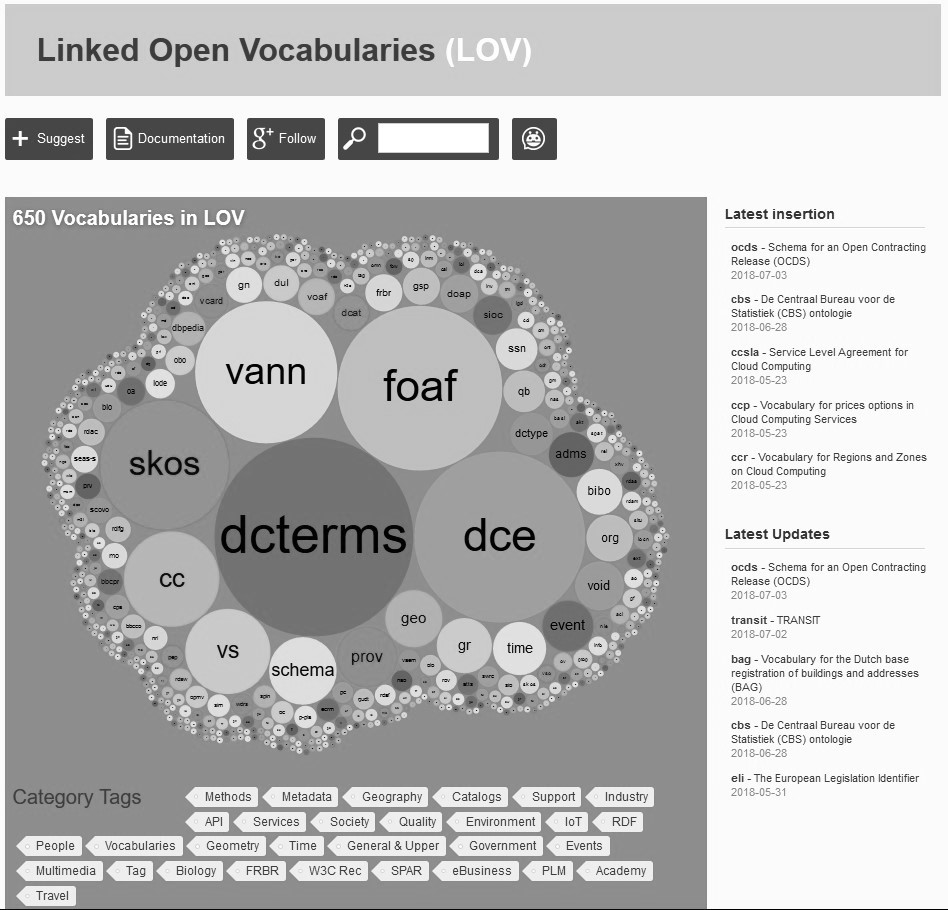
\includegraphics[width=5.0in]{media/ch5/figure-05-12.jpg}
    \caption{Linked Open Vocabularies (LOV) at OKFN.  From https://lov.linkeddata.es/, edited only for color. Licence https://creativecommons.org/licenses/by/4.0/}
    \label{fig:ch5.12}
\end{figure}

\hypertarget{cooking-a-web-of-linked-data-the-datatouille-metaphor}{%
\subsection{\texorpdfstring{Cooking a Web of linked data: the
\emph{Datatouille}
metaphor}{Cooking a Web of linked data: the Datatouille metaphor.  }}\label{cooking-a-web-of-linked-data-the-datatouille-metaphor}}

The overall process for producing and consuming linked data on the Web
may also be explained using a secret of ratatouille recipe. To obtain a
perfect ratatouille dish as cooked in the south of France one of the
tricks is to cook each vegetable separately (stage 1). Once each one is
properly cooked, the chef mixes them and cooks the ratatouille as one
dish (stage 2). Ratatouille is such a versatile dish, that it can be
used as an ingredient for other dishes such as (stage 3).

Preparing, publishing and (re)using linked data has a lot in common with
this process. Each data source is massaged and prepared separately by
its owner. Each data provider has their own
constraints in terms of data selection (sensitivity, anonymity, etc.),
data set features (velocity, volume, etc.) and data infrastructure
(legacy software, maintenance cost, etc.). Each source will therefore
cook its linked data separately (stage 1). Then anyone can use and link
to these published data and process them to produce new data: aggregated
data, statistics/mining/inference results, etc. (stage 2). In turn,
these new data become sources that their owners may publish as linked
data on the Web (stage 3).

\begin{figure}

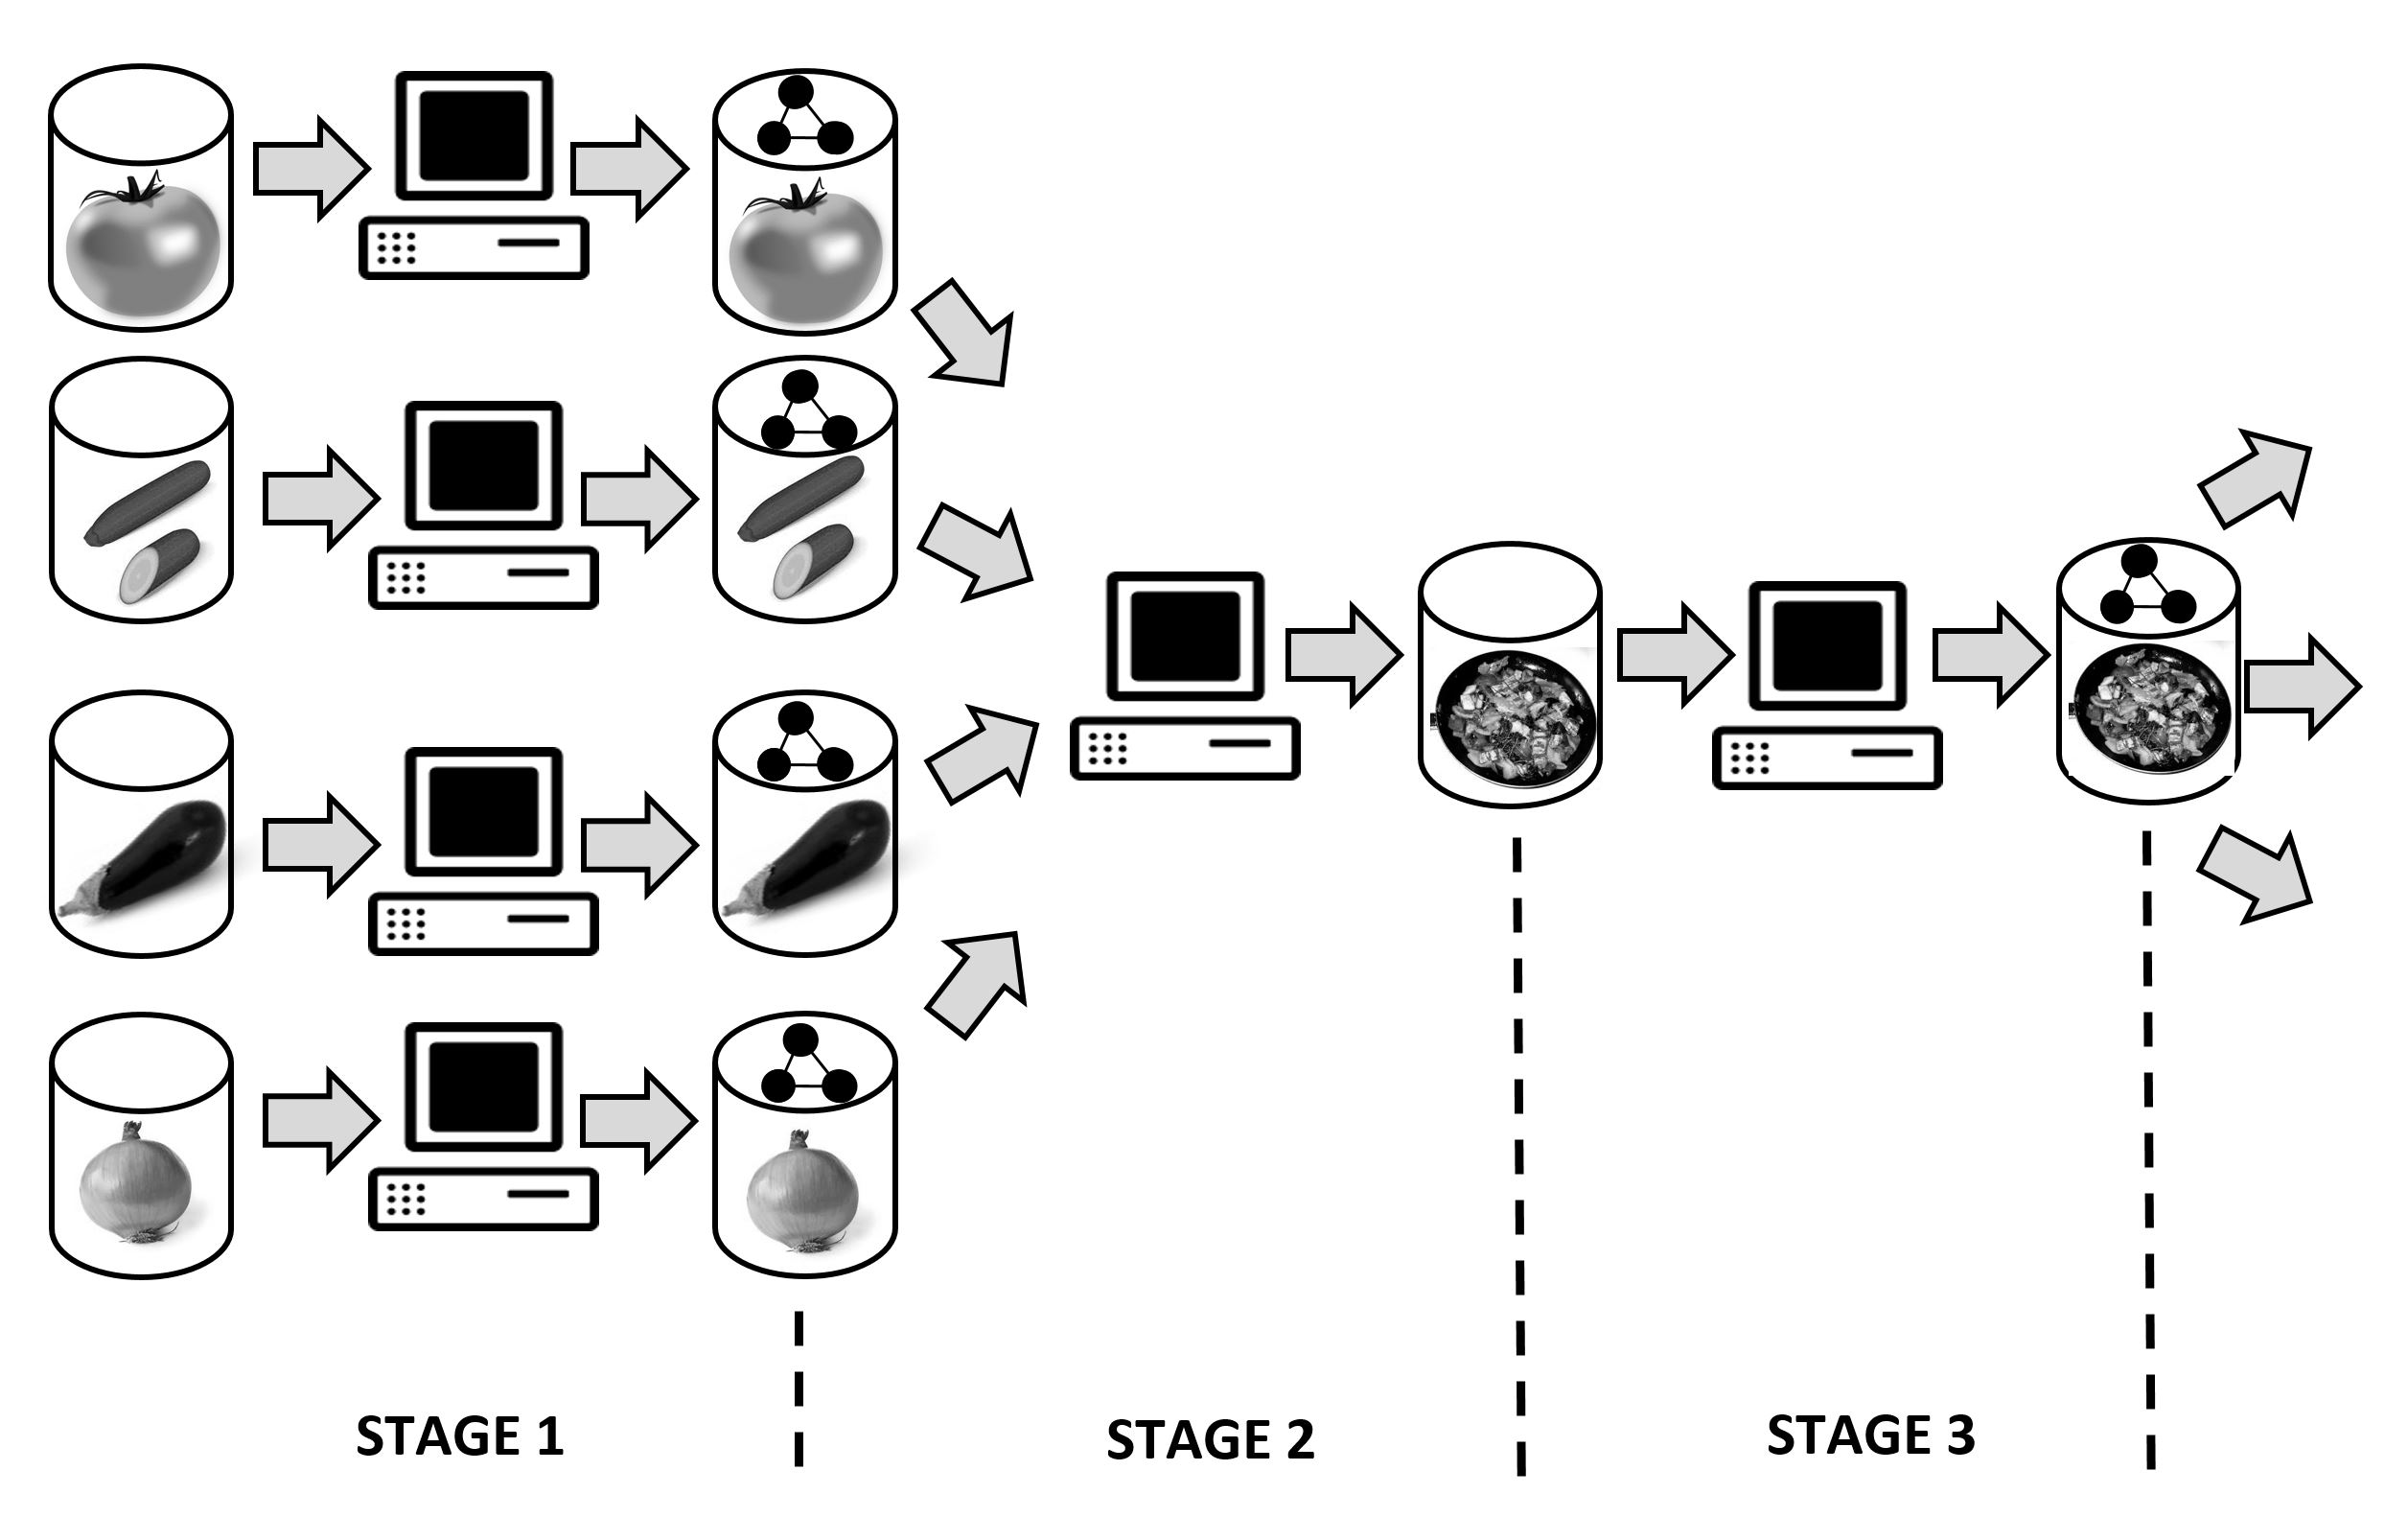
\includegraphics[width=5in]{media/ch5/figure-05-13x}
\label{fig:ch5.13x}
\caption{Three stages in producing linked data.}
\end{figure}

\hypertarget{linked-data-principles-in-a-mug}{%
\subsection{Linked data principles in a
mug}\label{linked-data-principles-in-a-mug}}

The W3C also found a way to summarize the linked data principles and had
it printed on mugs as what is called the 5-star deployment scheme for
Linked Data proposed by Tim Berners-Lee. The scheme is a cumulative list
of rules to lift Web data from one star to five stars. Each additional
rule to gain a star presumes the data meets the all of the previous
rules. The rules are given in figure~\ref{fig:ch5.13}, and they recommend that
data be available on the Web, in a non-proprietary structured format
using open W3C standards and linked to other data.

\begin{figure}
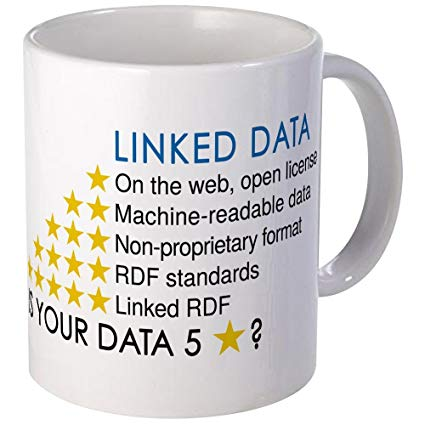
\includegraphics[width=3.5in]{media/ch5/figure-05-13.jpg}
\begin{quote}
$\star{}$ Data is available on the Web, in whatever format.

$\star{}\star{}$ Available as machine-readable structured data, (i.e., not a scanned
image).

$\star\star\star$ Available in a non-proprietary format, (i.e, CSV, not Microsoft
Excel).

$\star\star\star\star$ Published using open standards from the W3C (RDF and SPARQL).

$\star\star\star\star\star$ All of the above and links to other Linked Open Data.
\end{quote}
\caption{Linked data principles from the W3C}
\label{fig:ch5.13}
\end{figure}


\hypertarget{yet-another-cloud-for-the-web}{%
\subsection{Yet Another Cloud For the
Web}\label{yet-another-cloud-for-the-web}}

The term ``linked open data cloud'' or ``LOD Cloud'' does not refer to
the cloud paradigm of computer science but to of linked data sets
obtained by applying the linked data principles. This cloud is a graph
formed by nodes representing open data sets and edges indicating that the
data of two data sets are linked  the sense of Section~\ref{linking-rdf-data}, i.e. if one data set reuses some
identifiers from the other to identify the same resources (e.g.
persons, places, etc.). This cloud comprises only a small part the Web
of Data, made up of data sets that have registered at the Linked Open Data
Hub Web site at https://old.datahub.io/organization/lodcloud, 
which collects and curates their descriptions before
compiling them into the Linking Open Data cloud diagram as shown in
figure~\ref{fig:ch5.14}.

\begin{figure}
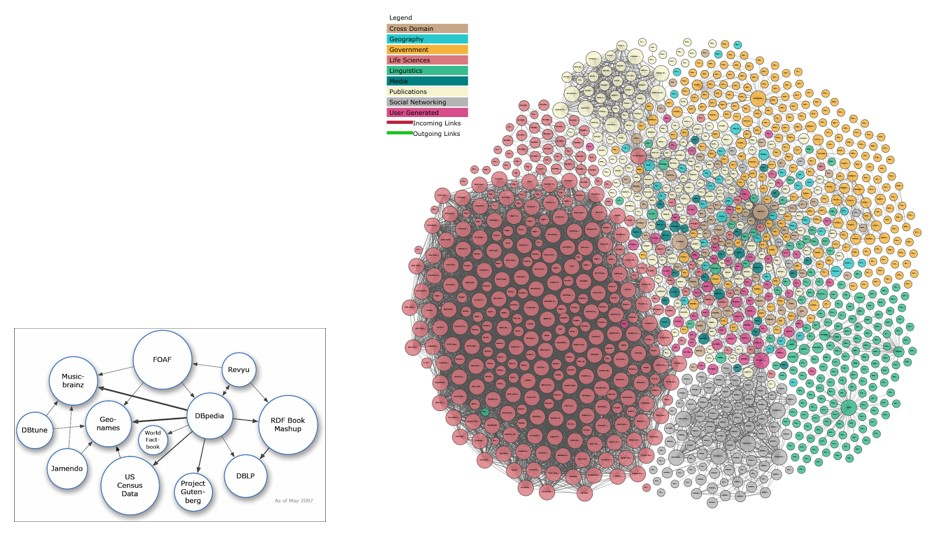
\includegraphics[width=5.0in]{media/ch5/figure-05-14.jpg}
\caption{\label{fig:ch5.14}Linking Open Data cloud diagrams\protect\footnotemark\ ten years apart from 2007 (left) and 2017 (right).  From The Linked Open Data Cloud from lod-cloud.net, edited for color.  License https://creativecommons.org/licenses/by/2.0/}
\end{figure}
\cite{lodcloudnet}

The 2017 edition of the diagram shown above shows a LOD cloud
aggregating 150 billion triples from nearly 3000 data sets. Each node
(circle) corresponds to a data set, some of them very large in their own
right. The different colors show different domains of application (e.g.
life sciences, publication, government, geography).

Some of the sources included in this cloud are well-known for being
central or historic.  We've seen most of these before:

\begin{itemize}
\item
  \emph{DBPedia}, described in Section~\ref{dbpedia} was one of the first reliable open sources
  of data and identifiers in
  the linked open data cloud. It is one of the pioneering sources and
  its encyclopedic nature makes it well-suited as a source of reference
  for other data sets.

\item
  \emph{Wikidata}, also described in Section~\ref{dbpedia}, is a close relative of DBpedia.  In contrast to
  DBpedia, Wikidata's approach is not to extract data
  from other sources but to directly edit and curate structured data in
  a Wiki manner.  This structured data sources can be queried to
  generate content such as tables or infoboxes in other sites. 

\item
  \emph{Geonames} is a free geographical database that covers all countries
  and, at the time of this writing, contains over eleven million place
  descriptions (countries, cities, regions, etc.) with their names and
  information including currency, population, language, area,
  geographical coordinates, etc.

\item
  \emph{UniProt} stands for Universal Protein Resource and is an international
  initiative to build and publish a comprehensive data set of protein
  sequences and annotations.
\end{itemize}



\hypertarget{the-linked-data-platform-architecture}{%
\subsection{The Linked Data Platform
architecture}\label{the-linked-data-platform-architecture}}

In the history of the development of the Web as an application architecture,
a great advance was made with the specification of 
\emph{Representational State Transfer} (\emph{REST}), a set of recommendations 
for how to organize and publicize a service on the Web.  
REST could be a topic of a book in its own right, but the basic 
structure of REST is that it ensures service
interoperability over the Web, based on accessing and manipulating
representations of resources through a small, uniform and predefined set of
operations (in particular, the standard HTTP methods \emph{GET},
\emph{PUT}, \emph{PATCH}, \emph{POST}, and \emph{DELETE}). A service
that complies with the REST principles is said to be \emph{RESTful}.

Following on the success of REST, the W3C has defined the \emph{Linked Data Platform} (LDP) \cite{Speicher:15:LDP}, which
specifies how web applications can publish, edit and delete data
resources using the HTTP protocol. LDP is a standardized specification of how to use REST
access to linked data, describing how to build clients and servers that
create, read, and write linked data resources.

Because  real applications  have to manage a variety of files and
data formats, LDP distinguishes two kinds of resources: resources with
an RDF representation (RDF descriptions) and resources using other
formats (e.g. HTML files, images, binary files).

In order to be able to add or remove resources from the Web, you need to
have some kind of data space in which to read and write these resources.
For this reason, LDP also introduces the notion of a \emph{container} to
group and manage resources.  A container is collections of resources; often the members of a container
are  homogeneous  (e.g. a collection of user profiles, a catalog of
book descriptions, an inventory of cars). LDP supports three kinds of
containers with varying levels of support for automation of the management of 
the resources in the container:

\begin{itemize}
    \item A
\emph{Basic Container} provides a simple containment vocabulary and
access mechanism. 

\item A \emph{Direct Container} supports the use of a
domain-specific membership assertions (e.g. assert a relation called
``author'' between all the resources of a collection of books and a
resource representing their author).

\item An \emph{Indirect Container} provides more precise control of the URIs of the domain-specific member
resources you create.

\end{itemize} 

LDP specifies the effect that each HTTP verb has on resources and
containers. Figure~\ref{fig:ch5.17} summarizes each case and shows how to use the standard HTTP verbs to 
remotely manage
resources and containers in an LDP-compliant platform. 


\begin{figure}
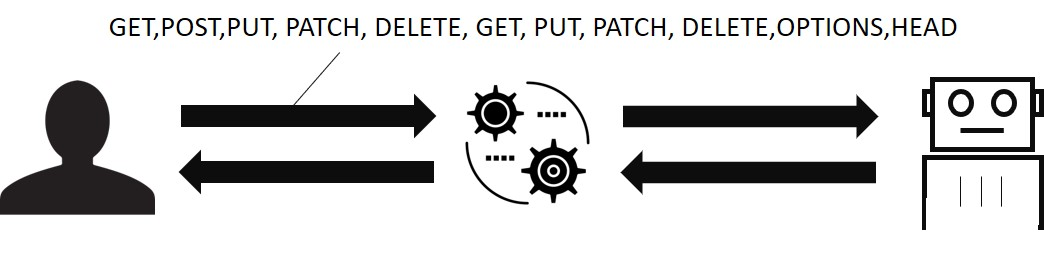
\includegraphics[width=5.0in]{media/ch5/figure-05-17.jpg}
\begin{tabular}{|lll|}
\hline
\textbf{Resource type} & \textbf{Method} & \textbf{Result}\tabularnewline
\hline\hline
Container & GET & Lists all the members of the container\tabularnewline
& POST & Create a new member of the container\tabularnewline
& PUT & Update the description of the container\tabularnewline
& PATCH & Partial update of the description of the
container\tabularnewline
& DELETE & Delete the container\tabularnewline
\hline
Any other resource type & GET & Retrieve a representation of the
resource\tabularnewline
& PUT & Update the resource description\tabularnewline
& PATCH & Partial update of the resource description\tabularnewline
& DELETE & Delete the resource description\tabularnewline
\hline\hline
Container or resource & OPTIONS & Discover the allowed operations over a
resource\tabularnewline
& HEAD & Only retrieve meta-information about a resource\tabularnewline
\hline
\end{tabular}
 \caption{The effects of HTTP verbs as specified in LDP\label{fig:ch5.17}}
\end{figure}


Figure~\ref{fig:ch5.18} shows the transcript of an HTTP request (lines 1-13) sent to a
container (/fabien/, line 1) on an LDP platform on a Web server
(inria.fr, line 2). The request uses the verb POST (line 1). As we saw in 
Figure~\ref{fig:ch5.17}, using the verb POST to a container creates a new member of that container. The
request provides the description of the RDF resource in Turtle
(serialization specified in line 4), and directly includes the data for
the new resource (lines 7-13). The response coming back from the server 
(lines
15-18) shows that the server accepted the request  (line 16), the
resource was created (also line 16), and the URI of the
newly created description is returned (line 17).

\begin{figure}

\begin{lstlisting}
1.	POST /fabien/ HTTP/1.1
2.	Host: inria.fr
3.	Link: <http://www.w3.org/ns/ldp#Resource>; rel="type"
4.	Content-Type: text/turtle
5.	Slug: foaf
6.	
7.	@prefix foaf: <http://xmlns.com/foaf/0.1/> .
8.	@prefix dc: <http://purl.org/dc/terms/> .
9.	<> a foaf:PersonalProfileDocument;
10.	   foaf:primaryTopic <#me> ;
11.    dc:title 'Fabien's FOAF profile' .
12.	<#me> a foaf:Person;
13.	   foaf:name 'Fabien Gandon' .
14.	 
15.	 
16.	HTTP/1.1 201 Created
17.	Location: http://inria.fr/fabien/foaf
18.	Link: <http://www.w3.org/ns/ldp#Resource>; rel="type"
19.	Content-Length: 0

\end{lstlisting}  
  \caption{Example of a POST request on an LDP container and its result   \label{fig:ch5.18}}
  \end{figure}

% Let's put a section in here about URIs in the enterprise.  What are the issues? 
% All of our own URIs are going be be local, 
% We aren't going to open them all up and make them available by FYN
% Nevertheless, we need to organize them, and know where to look for data
% We'll be in a Web Services setting (try not to say RESTful)
% This means that our URIs really are identifiers; we won't be resolving them, 
% except for the ones that are service calls
% Parameters sent via HTTP protocol (GET and POST) 
% 




\hypertarget{summary}{%
\section{SUMMARY}\label{summary:ch5}}

To weave a Web of linked data you must follow three rules: (1) use HTTP
URIs to name everything (2) provide descriptive information in
appropriate formats about the resources identified by these URIs every
time they are accessed, and (3) include, in these descriptions, links to
HTT URIs of other things. We have seen how to mint the URIs and how
HTTP can be used to negotiate the best answer when dereferencing a URI.
We showed examples of linked data resources on the Web today, and how they form
a Linked Data Cloud. 
Finally, we saw how
the Linked Data Platform (LDP) specification provides a standardized service
architecture and set of operations based on HTTP verbs to read and write
resources and resource descriptions on the Web of data.

\hypertarget{fundamental-concepts}{%
\subsection{Fundamental concepts}\label{fundamental-concepts}}

The following fundamental concepts were introduced in this chapter:

\begin{itemize}
\item
  \emph{\textbf{HTTP URI}}: a URI created to name anything but that
  uses the HTTP protocol.
\item
  \emph{\textbf{dereferencing}}: the process of resolving an HTTP URI to find information about 
  the resource it references. 
\item
  \emph{\textbf{content negotiation}} the process by which an HTTP server provides content in different forms when 
  resolving the
  same HTTP URI, based on client content specifications.  

\item 
  \emph{\texbf{Linked Data Platform (LDP)}}: a sest of recommendations about how web applications should 
  publish, edit and delete resources using the HTTP protocol.
\end{itemize}

